\capitulo{1}{Introducción}

Quiero comentar brevemente que la idea inicial para el proyecto no era la de crear una aplicación para dispositivos móviles. Si no que se pensó en otros trabajos previos a Flutter Games:

\begin{itemize}
	\item A finales del 2019 la idea era hacer el proyecto final de grado dentro de la empresa donde me encontraba haciendo las prácticas extracurriculares (ITCL). El trabajo consistía en una aplicación de reconocimiento de la mosca de la fruta en imágenes. Pero no prosperó.
	
	\item La siguiente propuesta de mis tutores fue la de trabajar con la herramienta \emph{Knime} junto con \emph{Moodle}. Dedique muchas horas a este proyecto, pero era de investigación y no me motivaba, por lo que se acabó descartando esta opción.
\end{itemize}

Finalmente, para no perder la convocatoria me decanté por hacer una aplicación Android mediante Flutter~\cite{wiki:flutter}. El porque de esta decisión es que la cuota de mercado para este sistema operativo es enorme~\cite{wiki:marketOS}, con un fuerte crecimiento hasta 2018 cuando se estabilizó. Actualmente es el líder del mercado como podemos ver en la siguiente imagen~\ref{fig:cuota}. 

También se debe remarcar que la cuota de mercado de los sistemas operativos tradicionales no para de descender, lo que implica que los móviles han venido para quedarse, pero no para sustituir a los ordenadores. Por lo que es una apuesta de futuro aprender el desarrollo de estas aplicaciones móviles, ya que la demanda es muy grande.

\begin{figure}[H]
	\centering
	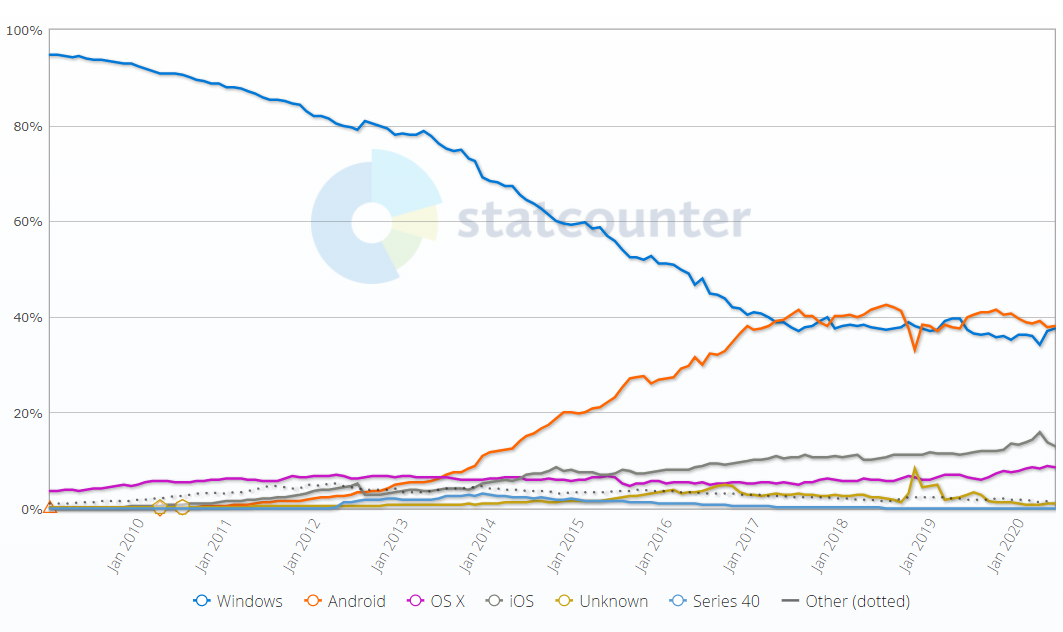
\includegraphics[width=1\textwidth]{teoria/cuota.png}
	\caption{Cuota de mercado}\label{fig:cuota}
\end{figure}

Básicamente me de decanté por Flutter porque permite la creación de aplicaciones para dos sistemas operativos (Android e iOS) y web. Todo ello programando en un mismo lenguaje, con las ventajas que esto conlleva, además al ser de Google, ofrece un gran soporte.

El contenido de la aplicación está basado en una colección de  videojuegos. De tal manera que esto sería el hilo conductor con el que poder tocar gran cantidad de tecnologías y aprender en profundidad del funcionamiento de Flutter.

\textbf{La colección inicial de juegos} se contará con estos dos primeros juegos:
\begin{itemize}
	\item \textbf{Cuatro en raya online}.
	\item \textbf{Snake o juego de la serpiente}
\end{itemize}

El juego de la serpiente contará con un ranking con el que poder compartir las puntuaciones. El objetivo es que entre los jugadores pueda haber un reto de ver quien consigue la mejor puntuación. Este ranking mostrará en orden descendente de mayor a menor puntuación obtenida por cada uno de los jugadores.  

En definitiva se desea hacer un juego lo más parecido a un producto real, subido en la \emph{Play Store}, con unos juegos iniciales (Snake y cuatro en raya online), publicidad para sacar rendimiento económicos y poder compartir la puntuación del snake en un ranking.
%% Terminar porque tenemos que explicar más cosas

\section{Estructura de la memoria}\label{estructura-de-la-memoria}

La memoria sigue la siguiente estructura:

\begin{itemize}
\tightlist
\item
  \textbf{Introducción:} breve descripción del problema a resolver y la
  solución propuesta. Estructura de la memoria y listado de materiales
  adjuntos.
\item
  \textbf{Objetivos del proyecto:} exposición de los objetivos que
  persigue el proyecto.
\item
  \textbf{Conceptos teóricos:} explicación de los conceptos
  teóricos clave para el entendimiento de la aplicación.
\item
  \textbf{Técnicas y herramientas:} listado de técnicas metodológicas y
  herramientas utilizadas para gestión y desarrollo del proyecto.
\item
  \textbf{Aspectos relevantes del desarrollo:} exposición de aspectos
  destacables que tuvieron lugar durante la realización del proyecto.
\item
  \textbf{Conclusiones y líneas de trabajo futuras:} conclusiones
  obtenidas tras la realización del proyecto y posibilidades de mejora o
  expansión de la solución aportada.
\end{itemize}

